\section{Durchführung}
\label{sec:Durchführung}
Die Messung der Reflektivität der Probe wird mittels
des D8-Labordiffraktometers
durchgefürt, das in der Abbildung \ref{fig:app} zu sehen ist.
\begin{figure}
  \centering
  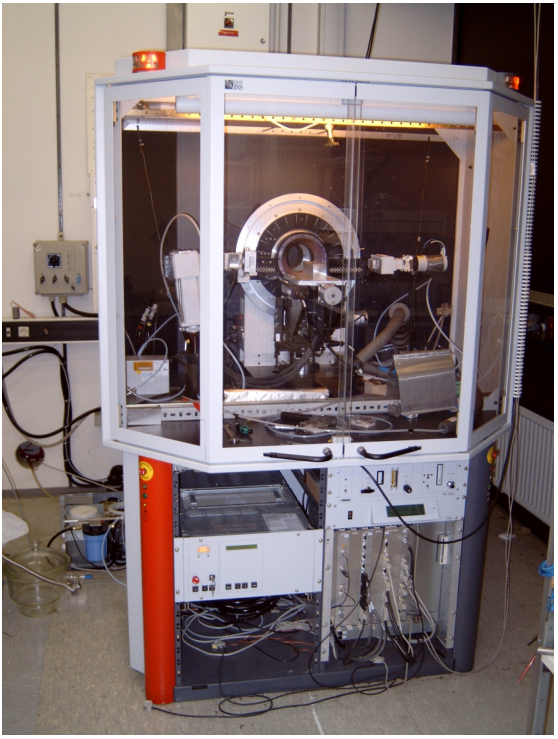
\includegraphics[width=0.6\textwidth]{bilder/apparatur.PNG}
  \caption{Das verwendete D8-Labordiffraktometers von der Firma Bruker AXS. \cite{sample}}
  \label{fig:app}
\end{figure}

Mit Hilfe des Gerätes kann sowohl der
Winkel der Röntgenröhre
als auch der Winkel des Detektor zum Probentisch
genau eingestellt werden. Desweitern ist es
möglich den Probentisch sowohl in x-Richtung als auch in
y,z-Richtung zu fahren.
Die Abbildung \ref{fig:anode_det} enthält eine genau
Ansicht zum Einen auf die
Röntgenröhre mit Blende und zum Anderen auf den Detektor des Gerätes.

\begin{figure}
  \centering
  \begin{subfigure}{0.5\textwidth}
  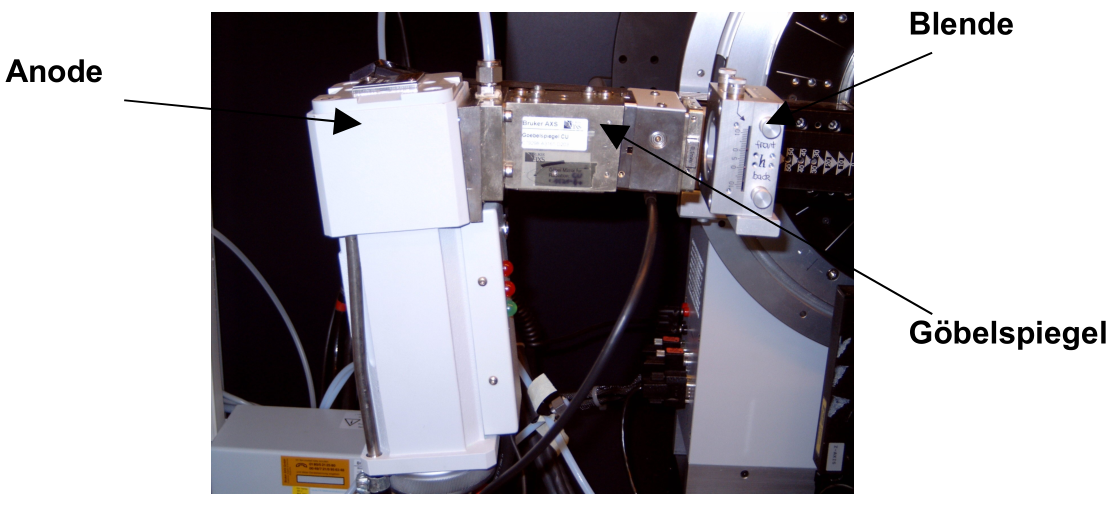
\includegraphics[width=0.9\textwidth]{bilder/anode.PNG}
  \caption{Röntgenröhre mit Blende und Göbelspiegel??.}
  \label{fig:anode}
\end{subfigure}
\begin{subfigure}{0.5\textwidth}
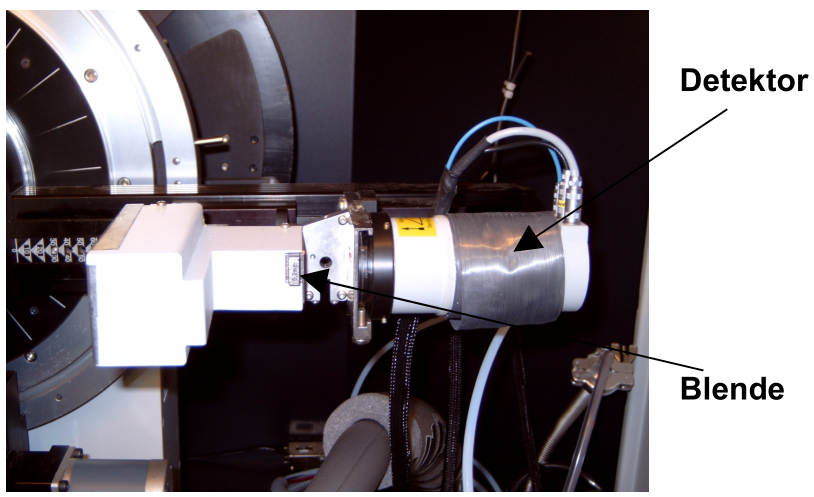
\includegraphics[width=0.9\textwidth]{bilder/detektor.PNG}
\caption{Detektor mit Blende.}
\label{fig:det}
\end{subfigure}
\caption{Röntgenröhre \ref{fig:anode} und Detektor \ref{fig:det} des D8-Labordiffraktometers. \cite{sample}}
\label{fig:anode_det}
\end{figure}

Die Röntgenröhre besitzt eine Kupferanode und wird mit einer Spannung von $\SI{40}{\kilo\volt}$
und einem Strom von $\SI{40}{\milli\ampere}$ betrieben.
Die Röntgenstrahlen der Röntgenröhre werden durch den Göbel Spiegel
gebündelt und monochromatisiert,
so dass der austretende Strahl eine Wellenlänge von
$\lambda=\SI{1.54}{\angstrom}$ besitzt.


\subsection{Justage des D8-Labordiffraktiometers}
\label{subsec:justage}
Bevor mit der Messung gestartet wird, wird das D8-Labordiffraktiometer
justiert. Dabei wird zwischen unterschiedliche Justageschritten Unterschieden.
% ?? strom und spannung hochfahren ??
% haben wir ja gar nichts mit zu tun gehabt


% Probe justieren
\paragraph{Probe justieren}


% Detektorscan
\paragraph{Detektorscan}


%  Z-Scan #1


% Rocking-Scan 0 grad


% Z-Scan #2


% Rocking-Scan 0.3 grad


% Z-Scan #3


% Rocking-Scan 1 grad




\subsection{Messung}
\label{subsec:messung}
Nachdem das Diffraktiometer justiert ist, wird anschließend
die eigentliche Messung durchgeführt.
Neben einer Messung mit Probe wird auch eine ohne durchgefürt,
um Untergrundsignale gegebenfalls abziehen zu können.

% Messung mit Probe
Bei diesem Messvorgang, wird eine Reflektivitätsscan vorgenommen.
Dabei werden $\alpha_{\text{i}}$ und der Winkel den Probe und Detektor einschließen nicht
variiert. Im verwendeten Programm, das die Messeinstellungen verwaltet, wird
"Omega / 2Theta" ausgewählt und ein Intervall von $\SI{0}{\degree}$ bis
$\SI{5}{\degree}$ gemessen.
Für die Schrittweite wird 0.005 % ?? prüfen ??
gewählt. Für die Geschwindgikeit des Scans werden $\SI{5}{\second}$ gewählt.


% Messung "Untergrund"
Um die störende Untergrundsignale aus den Messdaten entfernen zu können,
wird eine Messung ohne Probe durchgeführt. Diese kann bei der Auswertung
von den eigentlichen Messdaten abgezogen werden, um möglichst nur
Informationen über die Probe zu erhalten.
